%\part{Sampling and Reconstruction}
\section{Sampling and Reconstruction}
%\begin{frame}{Fourier Transform for Periodic Signals}
%    \begin{itemize}
%      \item We studied the Fourier transform for aperiodic signals. We can also develop Fourier transform representations for periodic signals, thus allowing us to consider both periodic and aperiodic signals within a unified context.
%      \item We can construct the Fourier transform of a periodic signal directly from its Fourier series representation. The resulting transform consists of a train of impulses in the frequency domain, with the areas of impulses proportional to the Fourier series coefficients.
%    \end{itemize}
%\end{frame}
%
%\begin{frame}[allowframebreaks]
%    Let us consider the signal $x(t)$ with Fourier transform $X(j\omega)$ that is a single impulse of area $2\pi$ at $\omega = \omega_0$:
%    \begin{equation*}
%        X(j\omega) = 2\pi \delta(\omega - \omega_0).
%    \end{equation*}
%    To determine the signal $x(t)$ we can apply the inverse Fourier transform relation
%    \pause
%    \mode<beamer>
%    {
%    \begin{equation*}
%        \begin{split}
%        x(t) &= \frac{1}{2\pi} \int_{-\infty}^{+\infty}2\pi \delta(\omega - \omega_0)e^{j\omega t}d\omega\\
%        &= e^{j\omega_0 t}.\\
%        \end{split}
%    \end{equation*}
%    More generally, if $X(j\omega)$ is of the form of a linear combination of impulses equally spaced in frequency, that is,
%    \begin{equation*}
%        X(j\omega) = \sum_{k=-\infty}^{+\infty}2\pi a_k \delta(\omega - k\omega_0).
%    \end{equation*}
%    then the application of the inverse Transform equation yields
%    \begin{equation*}
%        x(t) = \sum_{k=-\infty}^{+\infty}a_k e^{jk\omega_0 t}
%    \end{equation*}
%    }
%    This corresponds exactly to the Fourier \alert{series} representation of a periodic signal.\\
%    Thus the Fourier transform of a periodic signal with Fourier series coefficients $\{a_k\}$ can be interpreted as a train of impulses occurring at harmonically related frequencies for which the area of the impulse at the $k$th harmonic frequency $k\omega_0$ is $2\pi$ times the $k$the Fourier series coefficient $a_k$.
%\end{frame}
%
%
%\begin{frame}
%    \begin{example}
%        Consider the square wave.
%        \begin{center}
%            \begin{tikzpicture}[xscale=2]
	\draw (-3.5, 0) -- (3.5, 0) node [anchor=west] {$t$};
	\draw (0, 0) -- (0, 1.2) node [anchor=south] {$x(t)$};
	\foreach \x in {-3, -2, ..., 3}
	{
		\draw (\x, 0) -- ++(-0.2, 0) |- ++(0.4,1) -- ++ (0, -1);
		\draw (\x, 0.1) -- ++(0, -0.2);
		%\node at (\x, 0) [anchor=north] {\scriptsize $\x T$};
	}
	
	\foreach \x/\y in {-3/{-3T}, -2/{-2T}, -1/{-T}, 0/0, 1/{T},, 2/{2T}, 3/{3T}}
	{
		\draw (\x, 0) -- ++(-0.2, 0) |- ++(0.4,1) -- ++ (0, -1);
		\draw (\x, 0.1) -- ++(0, -0.2);
		\node at (\x, 0) [anchor=north] {\scriptsize $\y$};
	}
	\draw (-0.5, 0.1) -- ++(0, -0.2);
	\draw (0.5, 0.1) -- ++(0, -0.2);
	\node at (-0.5, 0) [anchor=north] {\scriptsize $-\dfrac{T}{2}$};
	\node at (0.5, 0) [anchor=north] {\scriptsize $\dfrac{T}{2}$};
	
	\node at (-0.2, 0) [anchor=north] {\scriptsize $-T_1$};
	\node at (0.2, 0) [anchor=north] {\scriptsize $T_1$};	
 
\end{tikzpicture}
%        \end{center}
%        \begin{enumerate}
%            \item Obtain the Fourier series coefficients $\{a_k\}$.
%            \item Obtain the Fourier transform of the signal.
%        \end{enumerate}
%    \end{example}
%\end{frame}
%
%\begin{frame}
%    \mode<beamer>
%    {
%        Fourier series coefficients:
%        \begin{equation*}
%            a_k = \frac{\sin k\omega_0 T_1}{\pi k}
%        \end{equation*}
%        \pause
%        Fourier transform\\
%        \begin{equation*}
%            X(j\omega) = \sum_{k=-\infty}^{+\infty}  2\frac{\sin k\omega_0 T_1}{ k}\delta (\omega - k\omega_0)
%        \end{equation*}
%
%    }
%\end{frame}
%
%
%\begin{frame}
%     \begin{center}
%        % \begin{tikzpicture}[scale=0.5]
% \begin{scope}	
%     \begin{axis}[
% 		y=4cm,
% 		x=1cm,
% 		 clip=false,
% 		 xmin=-10,xmax=10,
% 		 xlabel= $\omega$,
% 		 ylabel={$X(j\omega)$},
% 		 ymin=-0.5,ymax=1.2,
% 		 axis lines=middle,
%          	%xtick={-5, -4, ..., 5},
% 		 %ytick={-1, 1},
% 		 yticklabels=\empty,
% 		 xticklabels=\empty,
% 		 every axis x label/.style={at={(ticklabel* cs:1.05)}, anchor=west,},
% 		every axis y label/.style={at={(ticklabel* cs:1.05)}, anchor=south,},
%      ]
% 		%\addplot+[red, smooth, mark=none] table [x={n}, y={xn}] {periodic_square_fs_samples_of_envilope_gen.dat};
% 		\addplot [red, dashed, domain=-10:10, samples=200] plot{2*sin(deg(x)*2*pi/8*2)/(pi*x)};
% 		\addplot [thick, blue, ->, ycomb, domain=-10:10] plot{2*sin(deg(x)*2*pi/8*2)/(pi*x)};
% 		\node at (axis cs:0, 1) [anchor=east] { $\pi$ };
% 		\draw[latex-] (axis cs:pi/3, 0) --(axis cs:0.6,-0.3) node  [anchor=north] { $\pi/W$ } ;
% 		\draw[latex-] (axis cs:-pi/3, 0) --(axis cs:-0.6,-0.3) node  [anchor=north] { $-\pi/W$ } ;		
%     \end{axis}
% \end{scope}	
% \end{tikzpicture} 

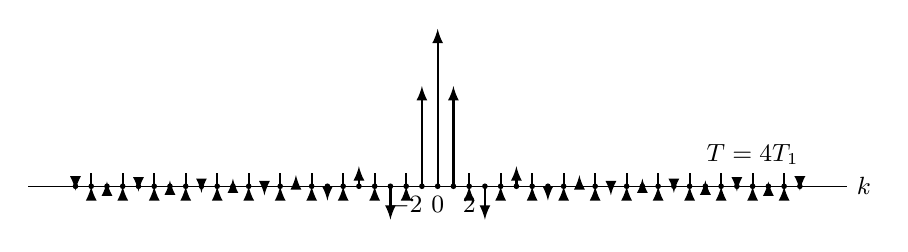
\begin{tikzpicture}[scale=0.4]
	\def\w{{-23,-22,-21,-20,-19,-18,-17,-16,-15,-14,-13,-12,-11,-10,-9,-8,-7,-6,-5,-4,-3,-2,-1,0,1,2,3,4,5,6,7,8,9,10,11,12,13,14,15,16,17,18,19,20,21,22,23}}
	\def\akmag{{-0.013840,0.000000,0.015158,-0.000000,-0.016753,0.000000,0.018724,-0.000000,-0.021221,0.000000,0.024485,-0.000000,-0.028937,0.000000,0.035368,-0.000000,-0.045473,0.000000,0.063662,-0.000000,-0.106103,0.000000,0.318310,0.500000,0.318310,0.000000,-0.106103,-0.000000,0.063662,0.000000,-0.045473,-0.000000,0.035368,0.000000,-0.028937,-0.000000,0.024485,0.000000,-0.021221,-0.000000,0.018724,0.000000,-0.016753,-0.000000,0.015158,0.000000,-0.013840}}


	\begin{scope}	
		\draw (-13, 0) -- (13,0) node[anchor=west] {\small $k$};
		\foreach \k in {-2, 0, 2}
		{
			\node at (\k/2, 0) [anchor=north] {\small $\k$};
		}
		%\node at (0,5) [anchor=south] {\small $Ta_k$};
		
		\foreach \k in {0,1, ..., 46}
		{
			\pgfmathparse{\w[\k]/2}
			\edef\wk{\pgfmathresult}
			\pgfmathparse{\akmag[\k]}
			\edef\akmagk{\pgfmathresult}	
			\draw[thick, -latex] (\wk, 0) -- ++(0,10*\akmagk);% node [anchor=south] {\small $\akmagk$};
			\ifthenelse{\lengthtest{0 pt = \akmagk pt}}{\draw[fill=black]  (\wk,0) circle (2pt);}{}
		}
			\node at (10, 1) {\small $T= 4T_1$};		
	\end{scope}
	\end{tikzpicture}
%    \end{center}
%\end{frame}
%
%\begin{frame}
%    \begin{example}
%        Sketch the Fourier transform of
%        \begin{enumerate}
%            \item $x(t) = \sin\omega_0 t$
%            \item $x(t) = \cos\omega_0 t$
%        \end{enumerate}
%    \end{example}
%\end{frame}
%
%
%\begin{frame}
%    \begin{example}
%        Obtain the Fourier transform of the impulse train given by
%        \begin{equation*}
%            x(t) = \sum_{k=-\infty}^{+\infty}  \delta(t - kT)
%        \end{equation*}
%        which is periodic with period $T$. Sketch.
%    \end{example}
%    \mode<beamer>
%    {
%        \begin{equation*}
%            a_k = \frac{1}{T}\int_{-T/2}^{T/2}\delta(t)e^{-jk\omega_0 t} dt \pause = \frac{1}{T}
%        \end{equation*}
%        \pause
%        \begin{equation*}
%            X(j\omega) = \dfrac{2\pi}{T}\sum_{k=-\infty}^{+\infty}\delta\left(\omega - \dfrac{2\pi k}{T}\right)
%        \end{equation*}
%
%    }
%\end{frame}

%\subsection{Sampling}

\begin{frame}{Introduction}
    \begin{itemize}
        \item Under ceratin conditions, a continuous-time (CT) signal can be completely represented by and recoverable from knowledge of its values at points equally spaced in time.
        \item These values are called \alert{samples}.
        \item This somewhat surprising property follows from a basic result that is referred to as the alert{sampling theorem}.
        \item Sampling theorem is extremely important, particulary as it forms the bridge between CT signals and discrete-time (DT) signals.
        \item Under ceratin conditions, a CT signal can be completely recovered from a sequence of its samples. This provides a mechanism for representing CT signals by a DT signal.
        \item We exploit sampling to convert a CT signal to a DT signal , process the DT signal using a DT system, and then convert back to CT.
    \end{itemize}
\end{frame}

\begin{frame}
    In general, in the absence of any additional information, we would not expect that a signal could be uniquely specified by a sequence of equally spaced samples.
    {
        \centering
        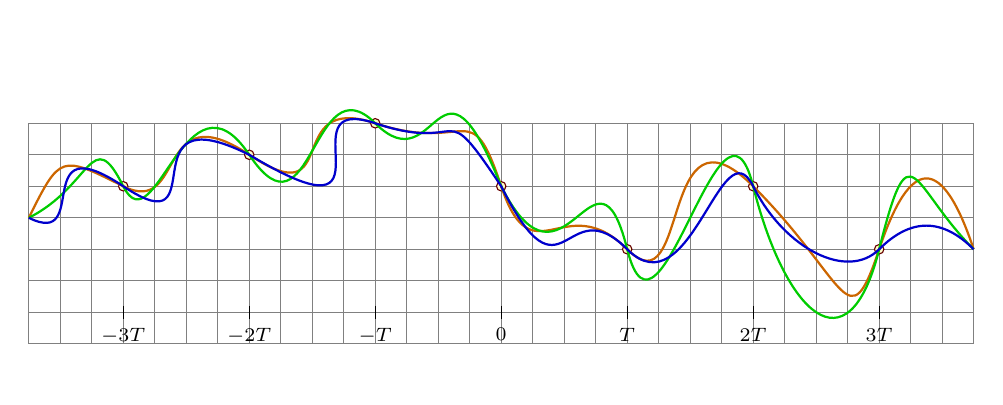
\begin{tikzpicture}[x=0.8cm, y = 0.8cm,
point/.style={circle, draw=red!40!black, fill=yellow!20, inner sep=0,  minimum size=0.12cm}
]
\draw (-7.5, 0) -- (7.5, 0);
\draw [help lines, step=0.5] (-7.5, -0.5) grid (7.5, 3);
\foreach \i/\s in {-6/{-3T}, -4/{-2T}, -2/{-T}, 0/0, 2/{T}, 4/{2T}, 6/{3T} }
{
	\draw (\i, 0.1) -- ++(0, -0.2) node [anchor=north] {\scriptsize $\s$};
}

\node [point] at  (-6,2) {};
\node [point] at  (-4,2.5) {};
\node [point] at  (-2,3) {};
\node [point] at  (0,2) {};
\node [point] at  (2,1) {};
\node [point] at  (4,2) {};
\node [point] at  (6,1) {};

\pause
\draw [thick, orange!80!black]
(-7.5,1.5)
.. controls (-7,2.5) and (-7,2.5) .. (-6,2)
.. controls (-5,1.5) and (-5.5,3.5) .. (-4,2.5)
.. controls (-2.5,1.5) and (-3.5,3.5) .. (-2,3)
.. controls (-0.5,2.5) and (-0.5,3.5) .. (0,2)
.. controls (0.5,0.5) and (1,2) .. (2,1)
.. controls (3,0) and (2.5,3.5) .. (4,2)
.. controls (5.5,0.5) and (5.5,-0.5) .. (6,1)
.. controls (6.5,2.5) and (7,2.5) .. (7.5,1);

\pause
\draw [thick, green!80!black]
(-7.5,1.5)
.. controls (-6.5,2) and (-6.5,3) .. (-6,2)
.. controls (-5.5,1) and (-5,4) .. (-4,2.5)
.. controls (-3,1) and (-3,4) .. (-2,3)
.. controls (-1,2) and (-1,4.5) .. (0,2)
.. controls (1,0) and (1.5,3) .. (2,1)
.. controls (2.5,-1) and (3.5,4) .. (4,2)
.. controls (4.5,0) and (5.5,-1) .. (6,1)
.. controls (6.5,3) and (6.5,2) .. (7.5,1);

\pause
\draw [thick, blue!80!black]
(-7.5,1.5)
.. controls (-6.5,1) and (-7.5,3) .. (-6,2)
.. controls (-4.5,1) and (-6,3.5) .. (-4,2.5)
.. controls (-1.5,1) and (-3.5,3.5) .. (-2,3)
.. controls (-0.5,2.5) and (-1,3.5) .. (0,2)
.. controls (1,0) and (1,2) .. (2,1)
.. controls (3,0) and (3.5,3) .. (4,2)
.. controls (4.5,1) and (5.5,0.5) .. (6,1)
.. controls (6.5,1.5) and (7,1.5) .. (7.5,1);

\end{tikzpicture} 
    }
    \par
    However, if the signal is band-limited---i.e., if its Fourier transform is zero outside a finite band of frequencies---and if the samples are taken sufficiently close together in relation to the highest frequency present in the signal, then the samples uniquely specify the signal, and we can reconstruct it perfectly.\par \par
    This result is known as the \alert{sampling theorem}.
\end{frame}

%\begin{frame}{Sampling}
%    \begin{itemize}
%        \item The sampling theorem, which is a relatively straightforward consequence of
%the modulation theorem, is elegant in its simplicity.
%        \item It states that a bandlimited time function can be exactly reconstructed from equally spaced samples provided that the sampling rate is sufficiently high---specifically, that it is greater than twice the highest frequency present in the signal.
%        \item A similar result holds for both continuous time and discrete time.
%        \item One of the important consequences of the sampling theorem is that it provides a mechanism for exactly representing a bandlimited continuous-time signal by a sequence of samples, that is, by a discrete-time signal.
%        \item The reconstruction procedure consists of processing the impulse train of samples by an ideal lowpass filter.
%    \end{itemize}
%\end{frame}


%\begin{frame}{Sampling Frequency and Aliasing}
%    \begin{itemize}
%        \item Assumption: the sampling frequency is greater than twice the highest frequency in the signal.
%        \item The reconstructing lowpass filter will always generate a reconstruction consistent with this constraint, even if the constraint was purposely or inadvertently violated in the sampling process.
%    \item Said another way, the reconstruction process will always generate a signal that is bandlimited to less than half the sampling frequency
%and that matches the given set of samples.
%    \item If the original signal met these constraints, the reconstructed signal will be identical to the original signal.
%    \item On the other hand, if the conditions of the sampling theorem are violated, then frequencies in the original signal above half the sampling frequency become reflected down to frequencies less than half the sampling frequency.
%    \item This distortion is commonly referred to as \alert{aliasing}, a name suggestive of the fact that higher frequencies (above half the sampling frequency) take on the alias of lower frequencies.
%    \end{itemize}
%\end{frame}






\begin{frame}{Impulse-Train Sampling}
    A convenient way to represent sampling of a CT signal at regular intervals is to use an impulse train multiplied by the CT signal $x(t)$ that we wish to sample.
    \begin{equation*}
        x_p(t) = x(t)p(t)
    \end{equation*}
    where
    \begin{equation*}
        p(t) = \sum_{n=-\infty}^{\infty}\delta(t-nT)
    \end{equation*}
    $p(t)$: sampling function, $T$: sampling period, $\omega_s = 2\pi/T$: sampling frequency.
    \begin{align*}
        x_p(t) &= x(t)\sum_{n=-\infty}^{+\infty} \delta(t - nT)\\
        &= \sum_{n=-\infty}^{+\infty} x(nT)\delta(t - nT)
    \end{align*}
\end{frame}


\begin{frame}

    \begin{columns}
        \begin{column}{0.6\textwidth}
            \mode<beamer>
            {
                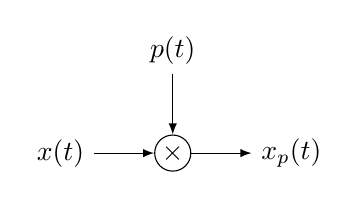
\begin{tikzpicture}[scale=0.5]
                	\draw (0,0) node (a) [anchor=east] {$x(t)$} ++(2,0) node (b) [draw, circle, inner sep=1pt] { $\times$} ;
                	\path (2,2) node (d) [anchor=south] {$p(t)$} ++(0, -2);
                	\path  (b)  ++(2,0) node (c) [anchor=west] {$x_p(t)$};
                	%\edge (a) -- (b);
                	
                	
                	\draw[-latex]  (a) edge (b);
                	\draw[-latex]  (b) edge (c);
                	\draw[-latex]  (d) edge (b);
                \end{tikzpicture}
                \pause

                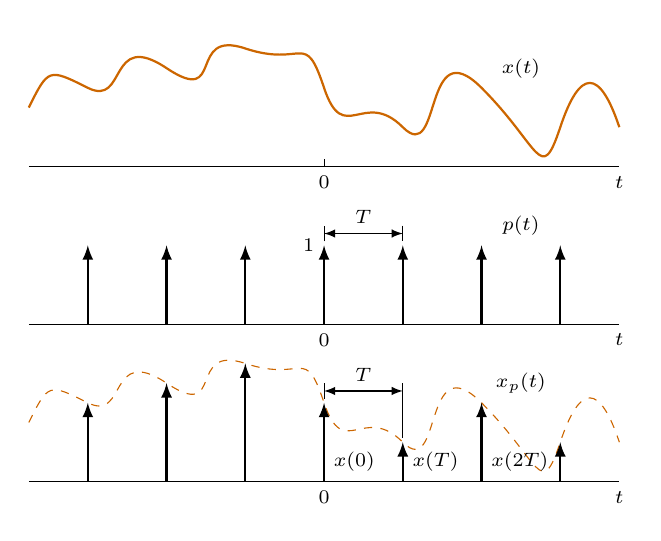
\begin{tikzpicture}[x=0.5cm, y=0.5cm]
	\draw (-7.5, 0) -- (7.5, 0) node [anchor=north] {\scriptsize $t$};
	\draw (0,0) -- ++(0,0.2);
	\node at (0,0)  [anchor=north] {\scriptsize $0$};
	\draw [thick, orange!80!black]
	(-7.5,1.5)
	.. controls (-7,2.5) and (-7,2.5) .. (-6,2)
	.. controls (-5,1.5) and (-5.5,3.5) .. (-4,2.5)
	.. controls (-2.5,1.5) and (-3.5,3.5) .. (-2,3)
	.. controls (-0.5,2.5) and (-0.5,3.5) .. (0,2)
	.. controls (0.5,0.5) and (1,2) .. (2,1)
	.. controls (3,0) and (2.5,3.5) .. (4,2)
	.. controls (5.5,0.5) and (5.5,-0.5) .. (6,1)
	.. controls (6.5,2.5) and (7,2.5) .. (7.5,1);	
	\node at (5,2)  [anchor=south] {\scriptsize $x(t)$};

\pause
\begin{scope}[yshift=-2cm]
	\draw (-7.5, 0) -- (7.5, 0) node [anchor=north] {\scriptsize $t$};	
	\node at (0,0)  [anchor=north] {\scriptsize $0$};	
	\foreach \i/\s in {-6/{-3T}, -4/{-2T}, -2/{-T}, 0/0, 2/{T}, 4/{2T}, 6/{3T} }
	{
		\draw[-latex, thick] (\i, 0) -- ++(0, 2);
	}
	\node at (5,2)  [anchor=south] {\scriptsize $p(t)$};	
	\node at (0,2)  [anchor=east] {\scriptsize $1$};	
	\draw (0, 2.1) -- ++(0, 0.4) ++(0, -0.2)  ++(2,0)   ++(0, 0.2) -- ++(0, -0.4) ;
	\draw[latex-latex] (0, 2.3) -- ++(2,0)  node[midway, above] {\scriptsize $T$};
\end{scope}

\pause
\begin{scope}[yshift=-4cm]
	\draw (-7.5, 0) -- (7.5, 0) node [anchor=north] {\scriptsize $t$};	
	\node at (0,0)  [anchor=north] {\scriptsize $0$};	
	\draw [orange!80!black, dashed]
	(-7.5,1.5)
	.. controls (-7,2.5) and (-7,2.5) .. (-6,2)
	.. controls (-5,1.5) and (-5.5,3.5) .. (-4,2.5)
	.. controls (-2.5,1.5) and (-3.5,3.5) .. (-2,3)
	.. controls (-0.5,2.5) and (-0.5,3.5) .. (0,2)
	.. controls (0.5,0.5) and (1,2) .. (2,1)
	.. controls (3,0) and (2.5,3.5) .. (4,2)
	.. controls (5.5,0.5) and (5.5,-0.5) .. (6,1)
	.. controls (6.5,2.5) and (7,2.5) .. (7.5,1);	
	\foreach \i/\s in {-6/{2}, -4/{2.5}, -2/{3}, 0/2, 2/{1}, 4/{2}, 6/{1} }
	{
		\draw[-latex, thick] (\i, 0) -- ++(0, \s);
	}
	\node at (5,2)  [anchor=south] {\scriptsize $x_p(t)$};	
	\draw (0, 2.1) -- ++(0, 0.4) ++(0, -0.2)  ++(2,0)   ++(0, 0.2) -- ++(0, -1.4) ;
	\draw[latex-latex] (0, 2.3) -- ++(2,0)  node[midway, above] {\scriptsize $T$};
	\node at (0,0.5) 	 [anchor=west] {\scriptsize $x(0)$};
	\node at (2,0.5) 	 [anchor=west] {\scriptsize $x(T)$};
	\node at (4,0.5) 	 [anchor=west] {\scriptsize $x(2T)$};	
\end{scope}
\end{tikzpicture} 
            }
        \end{column}
        \begin{column}{0.4\textwidth}
            \begin{equation*}
                x_p(t) = x(t)p(t)
            \end{equation*}
            \begin{equation*}
                p(t) = \sum_{n=-\infty}^{\infty}\delta(t-nT)
            \end{equation*}
            \begin{align*}
                x_p(t) &= x(t)\sum_{n=-\infty}^{+\infty} \delta(t - nT)\\
                &= \sum_{n=-\infty}^{+\infty} x(nT)\delta(t - nT)
            \end{align*}
        \end{column}
    \end{columns}

\end{frame}


\begin{frame}{Impulse-Train Sampling Cntd.}
    \begin{align*}
        X_p(j\omega)  &= \frac{1}{2\pi} \left[X(\omega)\ast P(\omega)\right]\\
        P(j\omega) &= \frac{2\pi}{T} \sum_{k=-\infty}^{+\infty}\delta\left(\omega- k\omega_s\right)
    \end{align*}
    \pause
    \begin{equation*}
        X_p(j\omega) = \frac{1}{T}\sum_{k=-\infty}^{+\infty} X\left(j(\omega- k\omega_s)\right)
    \end{equation*}
    \pause
    That is, $X_p(j\omega)$ is a periodic function of $\omega$ consiting of superposition of shifted replicas of $X(j\omega)$, scaled by $1/T$.
\end{frame}

\begin{frame}{}

    \begin{center}
            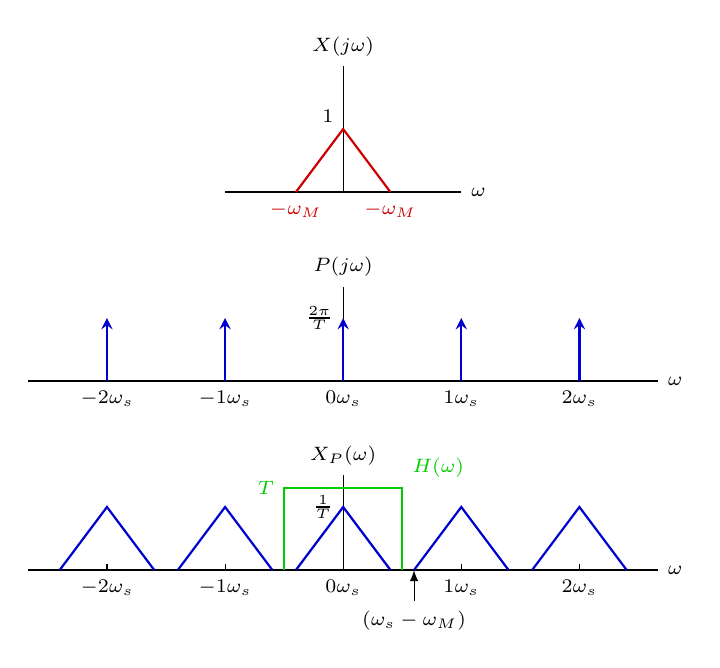
\begin{tikzpicture}[xscale=0.5, yscale=0.8]
    	\def\wm{1.2}
    	\def\ws{3.0}    	
        \draw (0,0) ++(-3,0) -- ++(6,0) node[anchor=west] {\scriptsize $\omega$};
        \draw (0,0) -- ++(0,2) node[anchor=south] {\scriptsize$X(j\omega)$};
        \draw[red!80!black, thick] (0,0) ++(-\wm,0) node[anchor=north] {\scriptsize$-\omega_M$} -- ++(\wm,1) -- +(\wm, -1) node[anchor=north] {\scriptsize$-\omega_M$};
        \node at (0, \wm) [anchor=east] {\scriptsize $1$};

        \begin{scope}[yshift=-3cm]
	        \draw (0,0) ++(-8,0) -- ++(16,0) node[anchor=west] {\scriptsize $\omega$};
	        \draw (0,0) -- ++(0,1.5) node[anchor=south] {\scriptsize$P(j\omega)$};
	        \foreach \w in {-2, -1, 0, 1, 2}
	        {
	            \draw[blue!80!black, thick, -stealth] (\w*\ws, 0) node[anchor=north, color=black] {\scriptsize $\w\omega_s$} -- ++(0, 1);
	        }
        	\node at (0, 1) [anchor=east] {\scriptsize $\frac{2\pi}{T}$};	
	\end{scope}
\pause
	
        \begin{scope}[yshift=-6cm]
	        \draw (0,0) ++(-8,0) -- ++(16,0) node[anchor=west] {\scriptsize $\omega$};
	        \draw (0,0) -- ++(0,1.5) node[anchor=south] {\scriptsize$X_P(\omega)$};
	        \foreach \w in {-2, -1, 0, 1, 2}
	        {
	
	            \draw[blue!80!black, thick] (\w*\ws, 0) ++(-\wm, 0) -- ++(\wm, 1) -- ++(\wm, -1);
	            \node at  (\w*\ws, 0) [anchor=north, color=black] {\scriptsize $\w\omega_s$};
	            \draw (\w*\ws, 0)  -- ++(0, 0.1);
	        }
	        \node at (0, 1) [anchor=east] {\scriptsize $\frac{1}{T}$};	
	        \draw[latex-] (\ws - \wm, 0) -- ++(0,-0.5) node  [anchor=north] {\scriptsize $(\omega_s - \omega_M)$};		
	\pause
 	\draw[thick, green!80!black] (-\ws/2, 0) -- ++(0,1.3) node [anchor=east] {\scriptsize $T$} -- ++(\ws, 0) node [anchor=south west] {\scriptsize $H(\omega)$} -- ++(0, -1.3);

	\end{scope}	

    \end{tikzpicture} 
    \end{center}
\end{frame}

\begin{frame}{}
\mode<beamer>
{
    \begin{center}
        \input{Figures/aliasing02}
    \end{center}
}
\end{frame}

\begin{frame}{}
\mode<beamer>
{
    \begin{center}
            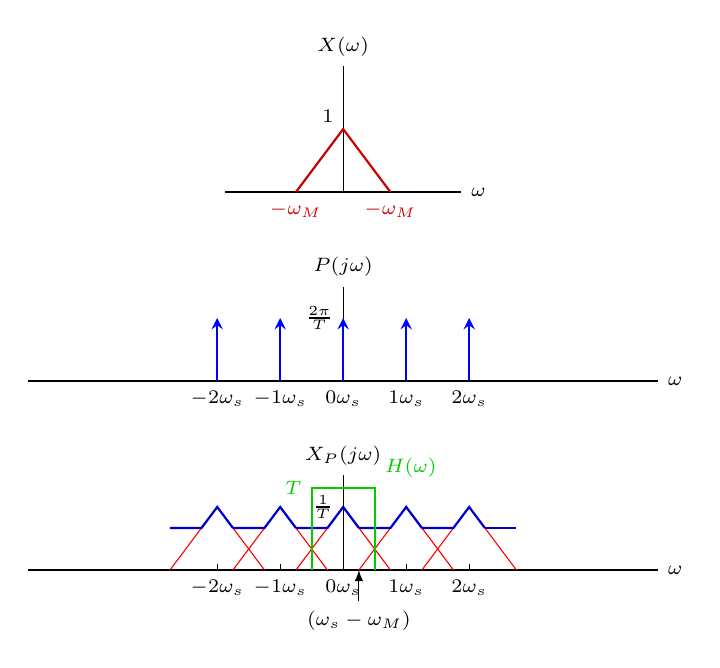
\begin{tikzpicture}[xscale=0.5, yscale=0.8]
    	\def\wm{1.2}
    	\def\ws{1.6}    	
        \draw (0,0) ++(-3,0) -- ++(6,0) node[anchor=west] {\scriptsize $\omega$};
        \draw (0,0) -- ++(0,2) node[anchor=south] {\scriptsize$X(\omega)$};
        \draw[red!80!black, thick] (0,0) ++(-\wm,0) node[anchor=north] {\scriptsize$-\omega_M$} -- ++(\wm,1) -- +(\wm, -1) node[anchor=north] {\scriptsize$-\omega_M$};
        \node at (0, \wm) [anchor=east] {\scriptsize $1$};        

        \begin{scope}[yshift=-3cm]
	        \draw (0,0) ++(-8,0) -- ++(16,0) node[anchor=west] {\scriptsize $\omega$};
	        \draw (0,0) -- ++(0,1.5) node[anchor=south] {\scriptsize$P(j\omega)$};
	        \foreach \w in {-2, -1, 0, 1, 2}
	        {
	            \draw[blue, thick, -stealth] (\w*\ws, 0) node[anchor=north, color=black] {\scriptsize $\w\omega_s$} -- ++(0, 1);
	        }
        	\node at (0, 1) [anchor=east] {\scriptsize $\frac{2\pi}{T}$};	
	\end{scope}
	
        \begin{scope}[yshift=-6cm]
	        \draw (0,0) ++(-8,0) -- ++(16,0) node[anchor=west] {\scriptsize $\omega$};
	        \draw (0,0) -- ++(0,1.5) node[anchor=south] {\scriptsize$X_P(j\omega)$};
		\def\tantheta{1/\wm}	
	        \foreach \w in {-2, -1, 0, 1, 2}
	        {
	
	            \draw[red, red] (\w*\ws, 0) ++(-\wm, 0) -- ++(\wm, 1) -- ++(\wm, -1);
	            \node at  (\w*\ws, 0) [anchor=north, color=black] {\scriptsize $\w\omega_s$};
	            \draw (\w*\ws, 0)  -- ++(0, 0.1);

	            \draw [blue!80!black, thick]  (\w*\ws - \wm, {(2*\wm - \ws)*\tantheta})  -- ++({(2*\wm - \ws)}, 0) -- ++({\ws - \wm)},{(\ws - \wm)*\tantheta}) -- ++({\ws - \wm)},{-(\ws - \wm)*\tantheta});
	
	        }
	            \draw [blue!80!black, thick]  (3*\ws - \wm, {(2*\wm - \ws)*\tantheta})  -- ++({(2*\wm - \ws)}, 0);
	        \node at (0, 1) [anchor=east] {\scriptsize $\frac{1}{T}$};	
	        \draw[latex-] (\ws - \wm, 0) -- ++(0,-0.5) node  [anchor=north] {\scriptsize $(\omega_s - \omega_M)$};	
\pause
 	\draw[thick, green!80!black] (-\ws/2, 0) -- ++(0,1.3) node [anchor=east] {\scriptsize $T$} -- ++(\ws, 0) node [anchor=south west] {\scriptsize $H(\omega)$} -- ++(0, -1.3);

			
		\end{scope}	

    \end{tikzpicture} 
    \end{center}
}
\end{frame}


\begin{frame}{Sampling Theorem}
    If $\omega_M < (\omega_s - \omega_M)$, or equivalently $\omega_s > 2\omega_M$, there is no overlap between shifted replicas of $X(j\omega)$. If $\omega_s > 2\omega_M$, $x(t)$ can be recovered exactly from $x_p(t)$ by means of a lowpass filter with gain $T$ and a cutoff frequency greater than $\omega_M$ and less than $\omega_s - \omega_M$.
    \begin{theorem} \end{theorem}
    Let $x(t)$ be a band-limited signal with $X(j\omega) = 0$ for $|\omega| > \omega_M$. Then $x(t)$ is uniquely determined by its samples $x(nT), \: n = 0, \pm 1, \pm 2, \dots$, if
    \begin{equation*}
        \omega_2 > 2\omega_M,
    \end{equation*}
    where $\omega_2 = 2\pi/T$\par
    Given these samples, we can reconstruct $x(t)$ by generating a periodic impulse train in which successive impulses have amplitudes that are successive sample values, The impulse train is then passed through an ideal lowpass filter with gain $T$ and cutoff frequency greater than $\omega_M$ and less than $\omega_s - \omega_M$. the resulting output signal will exactly equal $x(t)$.
        

\end{frame}



\begin{frame}{}
    \begin{center}
        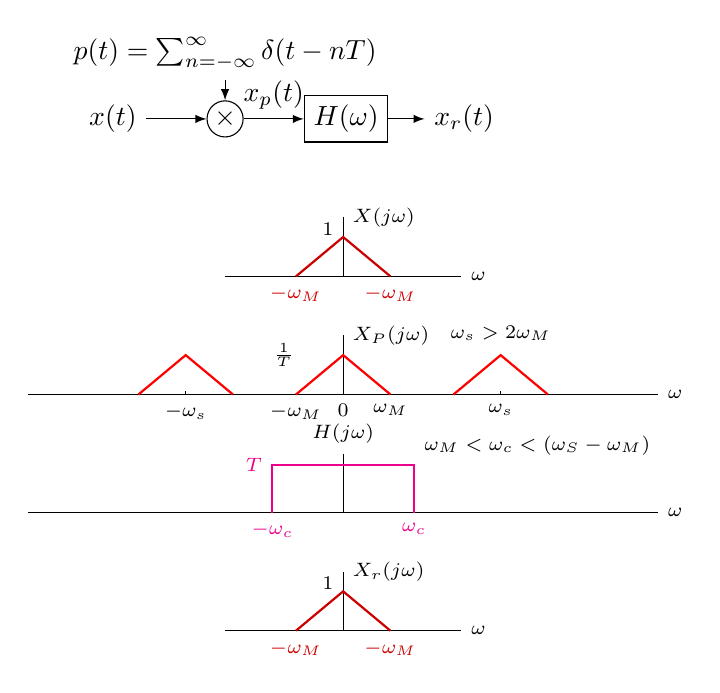
\begin{tikzpicture}[scale=0.5]
	\draw (0,0) node (a) [anchor=east] {$x(t)$} ++(2,0) node (b) [draw, circle, inner sep=1pt] { $\times$} ;
	\path (2,1) node (d) [anchor=south] {$p(t) = \sum_{n=-\infty}^{\infty}\delta(t-nT)$} ++(0, -2);
	\path  (b)  ++(2,0) node (c) [anchor=west, draw, rectangle, minimum height = 0.5cm] {$H(\omega)$};
	\path (c) ++(3,0) node (e) {$x_r(t)$};
	%\edge (a) -- (b);
	
	
	\draw[-latex]  (a) edge (b);
	\draw[-latex]  (b) edge node[above] {$x_p(t)$}(c) ;
	\draw[-latex]  (d) edge (b);
	\draw[-latex]  (c) edge (e);
    	\def\wm{1.2}
    	\def\ws{4.0}
    	\def\wc{3.6}

        \begin{scope}[yshift=-4cm, xshift=5cm]
            \draw (0,0) ++(-3,0) -- ++(6,0) node[anchor=west] {\scriptsize $\omega$};
            \draw (0,0) -- ++(0,1.5) node[anchor=west] {\scriptsize$X(j\omega)$};
            \draw[red!80!black, thick] (0,0) ++(-\wm,0) node[anchor=north] {\scriptsize$-\omega_M$} -- ++(\wm,1) -- +(\wm, -1) node[anchor=north] {\scriptsize$-\omega_M$};
            \node at (0, \wm) [anchor=east] {\scriptsize $1$};
        \end{scope}   	

        \begin{scope}[yshift=-7cm, xshift=5cm]
	        \draw (0,0) ++(-8,0) -- ++(16,0) node[anchor=west] {\scriptsize $\omega$};
	        \draw (0,0) -- ++(0,1.5) node[anchor=west] {\scriptsize $X_P(j\omega)$};
	        \foreach \w/\l in { -1/-\omega_s, 0/0, 1/\omega_s}
	        {
	
	            \draw[red, thick] (\w*\ws, 0) ++(-\wm, 0) -- ++(\wm, 1) -- ++(\wm, -1);
	            \node at  (\w*\ws, 0) [anchor=north, color=black] {\scriptsize $\l$};
	            \draw (\w*\ws, 0)  -- ++(0, 0.1);
	        }
	        \node [anchor=north] at (-\wm, 0) {\scriptsize$-\omega_M$};
	        \node [anchor=north] at (\wm, 0) {\scriptsize$\omega_M$};	
	        \node [anchor=north] at (\ws, 2) {\scriptsize$\omega_s > 2\omega_M$};	
	        \node [anchor=east, xshift=-0.5cm] at (0, 1) {\scriptsize$\frac{1}{T}$};	     	


	\end{scope}	
	
        \begin{scope}[yshift=-10cm, xshift=5cm]
	        \draw (0,0) ++(-8,0) -- ++(16,0) node[anchor=west] {\scriptsize $\omega$};
	        \draw (0,0) -- ++(0,1.5) node[anchor=south] {\scriptsize$H(j\omega)$};

 \draw[thick, magenta] (-\wc/2, 0) node [anchor=north] {\scriptsize $-\omega_c$} --  ++(0, 1.2) node [anchor=east] {\scriptsize $T$}  -- ++(\wc, 0)  node [anchor=south west, black] {\scriptsize $\omega_M< \omega_c < (\omega_S - \omega_M)$} -- ++(0, -1.2) node [anchor=north] {\scriptsize $\omega_c$} ;

	\end{scope}	

	        \begin{scope}[yshift=-13cm, xshift=5cm]
            \draw (0,0) ++(-3,0) -- ++(6,0) node[anchor=west] {\scriptsize $\omega$};
            \draw (0,0) -- ++(0,1.5) node[anchor=west] {\scriptsize$X_r(j\omega)$};
            \draw[red!80!black, thick] (0,0) ++(-\wm,0) node[anchor=north] {\scriptsize$-\omega_M$} -- ++(\wm,1) -- +(\wm, -1) node[anchor=north] {\scriptsize$-\omega_M$};
            \node at (0, \wm) [anchor=east] {\scriptsize $1$};
        \end{scope}

\end{tikzpicture} 
    \end{center}
\end{frame}

\begin{frame}{Discrete-Time Processing of Continuous-Time Signals}
    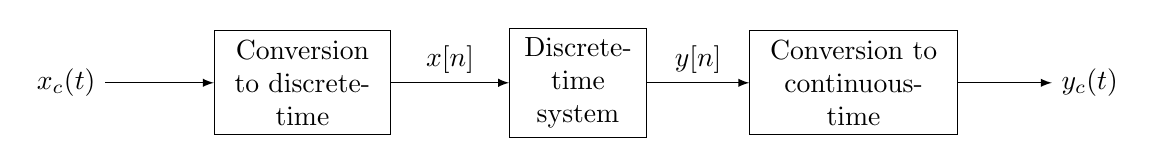
\begin{tikzpicture}
	\node (a) at (0,0) { $x_c(t)$};
	\path (a) -- ++(3,0) node[text width=2cm, draw, align=center] (b) {Conversion to discrete-time}  -- ++(3.5,0) node[text width=1.5cm, draw, align=center] (c) {Discrete-time system}  -- ++(3.5,0) node[text width=2.4cm, draw, align=center] (d) {Conversion to continuous-time}  -- ++(3,0) node (e) { $y_c(t)$};
	\draw[-latex] (a) edge (b);
	\draw[-latex] (b) edge  node[above] {$x[n]$}(c);
	\draw[-latex] (c) edge  node[above] {$y[n]$}(d);
	\draw[-latex] (d) edge  (e);
\end{tikzpicture} 
\end{frame}

\begin{frame}{}
\begin{columns}
    \begin{column}{0.5\textwidth}
        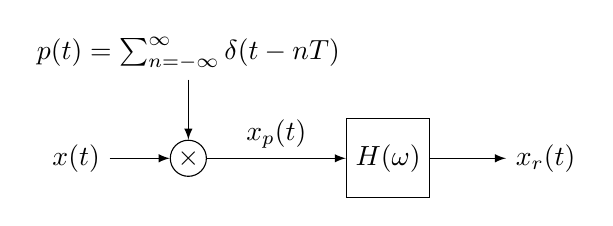
\begin{tikzpicture}[scale=0.5]
        	\draw (0,0) node (a) [anchor=east] {$x(t)$} ++(2,0) node (b) [draw, circle, inner sep=1pt] { $\times$} ;
        	\path (2,2) node (d) [anchor=south] {$p(t) = \sum_{n=-\infty}^{\infty}\delta(t-nT)$} ++(0, -2);
        	\path  (b)  ++(4,0) node (c) [anchor=west, draw, rectangle, minimum height = 1cm] {$H(\omega)$};
        	\path (c) ++(4,0) node (e) {$x_r(t)$};
        	\draw[-latex]  (a) edge (b);
        	\draw[-latex]  (b) edge node[above] {$x_p(t)$}(c) ;
        	\draw[-latex]  (d) edge (b);
        	\draw[-latex]  (c) edge (e);
        \end{tikzpicture}
    \end{column}
    \begin{column}{0.5\textwidth}
        \begin{align*}
            x_p(t) &= x(t)p(t)\\
            &= x(t)\sum_{n=-\infty}^{\infty}\delta(t-nT)\\
                &=\sum_{n=-\infty}^{\infty}x(nT)\delta(t-nT)
        \end{align*}

        \begin{align*}
            x_r(t) &= x_p(t)\ast h(t)\\
            &= \sum_{n = -\infty}^{+\infty} x(nT)h(t-nT)\\
        \end{align*}
    \end{column}
\end{columns}



\end{frame}

